\subsection{Mixed Design Model} 

Previously we used block design that has too long of duration, and therefore
unable to explain much of the variation in the BOLD signals. We revised
convolution of stimulus using a finer and higher resolution on time. With trials
within task blocks convolved and included in the design matrix, we expect the
result from linear regression have higher explanatory power. However, we need to
be cautious because the task block conditions (conditions 1, 4, and 5) are
likely to have colinearity problem with the trial conditions (conditions 2 and 3).

Figure \ref{fig:mixDM} shows the new design matrix has dimensions $133 \times 7$, 
where the first 6 columns are the convolved neural responses and the last column is 
theconstant.  

\begin{figure}[!h] 
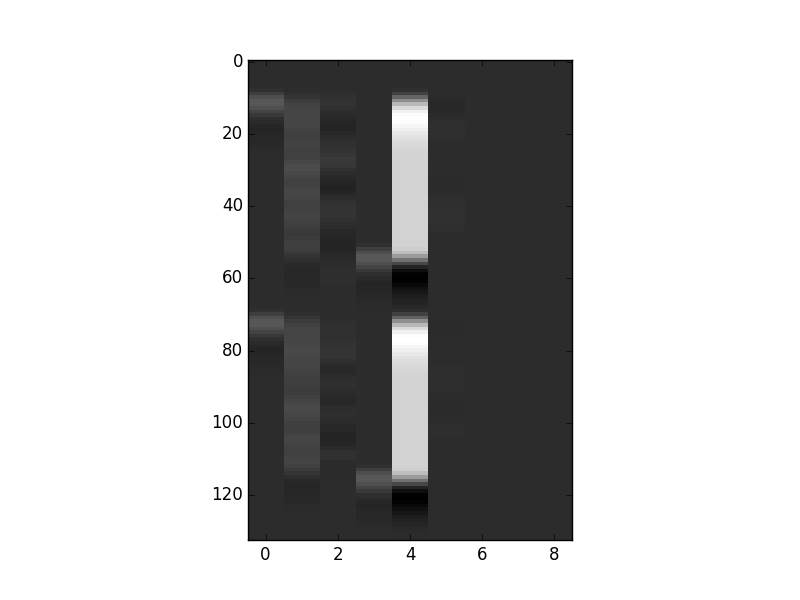
\includegraphics[scale=0.45]{full_design_mat} 
\centering
\caption{Design Matrix of Mixed Design\label{fig:mixDM}}
\end{figure}

\subsubsection{Mixed Model Linear Regression Results} 

With the $133 \times 7$ mixed model design matrix, we obtained 6 beta estimates
for each voxel using GLM. We perform t-test on each voxel, where the null
hypothesis claims that $\beta_1 + \beta_2 + \beta_3 + \beta_4 + \beta_5 +
\beta_6= 0$. Figure \ref{fig:mixMF} shows the statistical parametric maps. Each 
significant voxel is color-coded according to the size of its beta value, t value and p 
value. Since we are making multiple comparisons, we use the Bonferroni correction
for setting threshold. Using 0.05/133 as the threshold, we found a number of voxels 
near the center of the brain to be significant. The mean MRSS across all voxels 
using all 6 study conditions is 2041.804.

\begin{figure}[!h]
\begin{subfigure}{.5\textwidth}
  \centering
  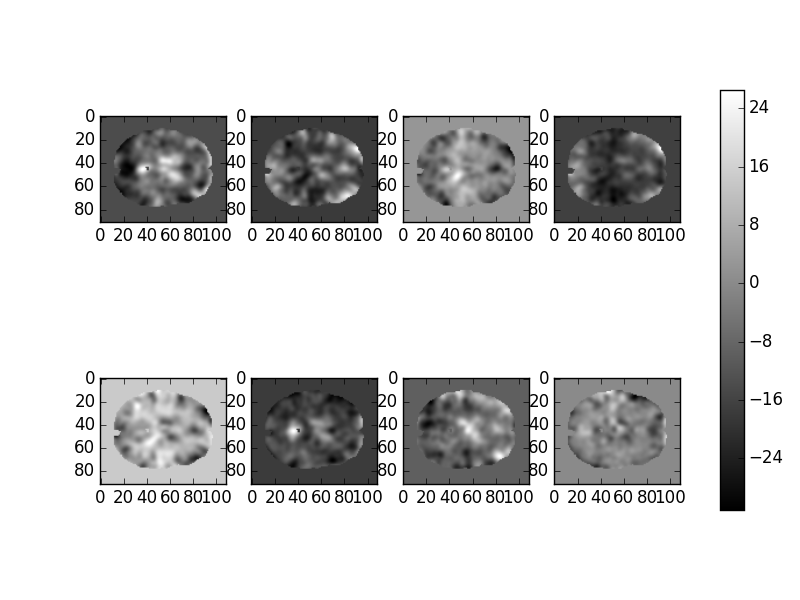
\includegraphics[scale=0.35]{full_beta}
  \caption{$\beta$ Map ($\beta_1, \ldots, \beta_6$)}
\end{subfigure}%
\begin{subfigure}{.4\textwidth}
  \centering
  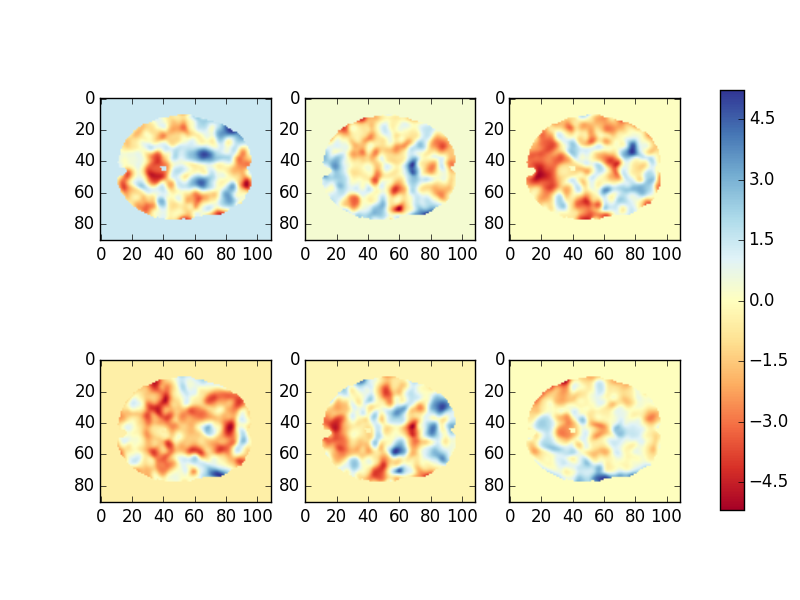
\includegraphics[scale=0.35]{full_t_map}
  \caption{t Map}
\end{subfigure}
\begin{subfigure}{.5\textwidth}
  \centering
  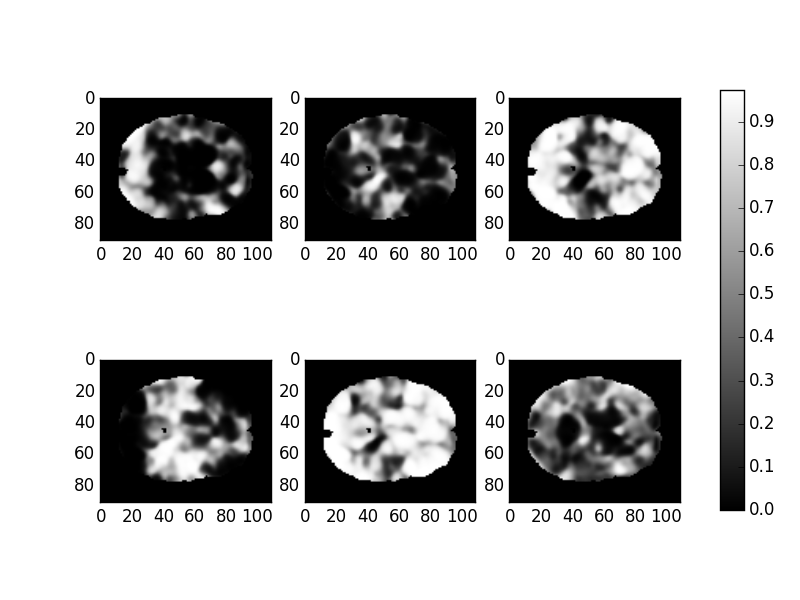
\includegraphics[scale=0.35]{full_p_map}
  \caption{p Map}
\end{subfigure}%
\begin{subfigure}{.5\textwidth}
  \centering
  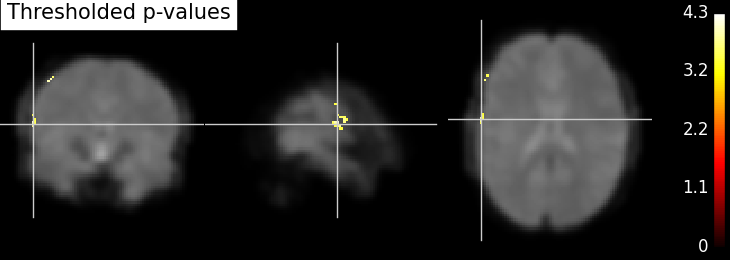
\includegraphics[scale=0.35]{full_sig_p_map}
  \caption{Significant p Map} 
\end{subfigure}
\caption{Mixed Model Parametric Maps\label{fig:mixMF}}
\end{figure}

\subsubsection{Temporal Smoothing}

To reduce noise and improve signal in the fMRI data, we attempted smoothing of
the fMRI data. We experimented with smoothing temporally using discrete cosine
transformations. We added a set of discrete cosine transformation basis to the
design matrix to filter out the low frequency noise present in the BOLD signal. This 
result in a larger design matrix of dimensions $133 \times 14$, which included the 
discrete cosine transformation basis.

As the block model and the mixed model, we used GLM to obtain 6 betas of interest.
We perform t-test on each voxel, where the null hypothesis claims that  $\beta_1
+ \beta_2 + \beta_3 + \beta_4 + \beta_5 + \beta_6= 0$. The mean MRSS across all
voxels using all 6 study conditions is 2033.76. The mean MRSS is smaller than
the mixed model, but we cannot conclude that this model is better yet. There are no 
voxels that are significant at the Bonferroni corrected threshold. We raised our
conservative threshold to about 0.05/110, and there are two voxels that are
significant.

\begin{figure}[!h]
\begin{subfigure}{.5\textwidth}
  \centering
  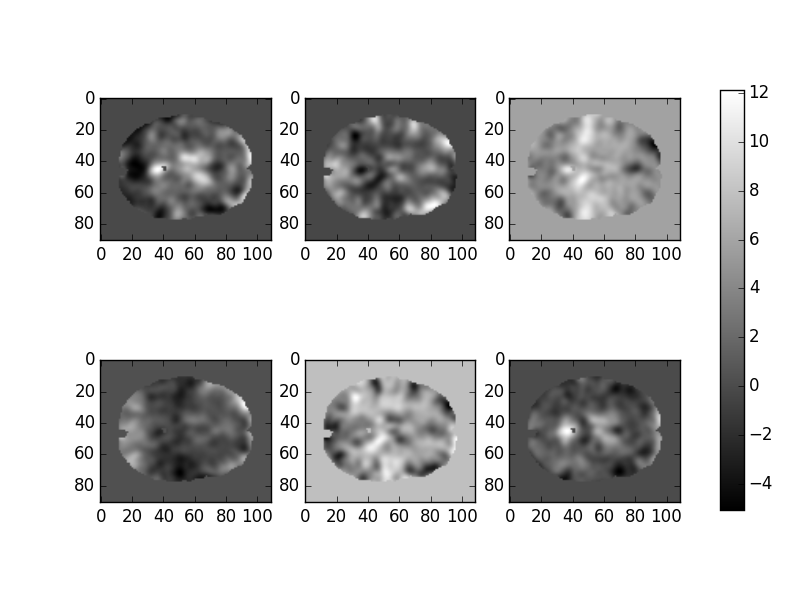
\includegraphics[scale=0.35]{dct_beta}
    \caption{$\beta$ Map ($\beta_1, \ldots, \beta_6$)}
\end{subfigure}%
\begin{subfigure}{.4\textwidth}
  \centering
  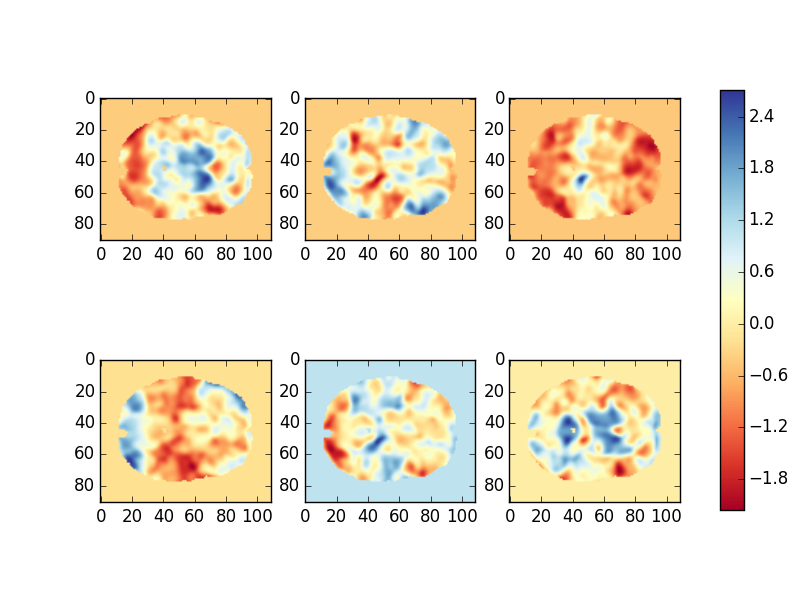
\includegraphics[scale=0.35]{dct_t_map}
  \caption{t Map}
\end{subfigure}
\begin{subfigure}{.5\textwidth}
  \centering
  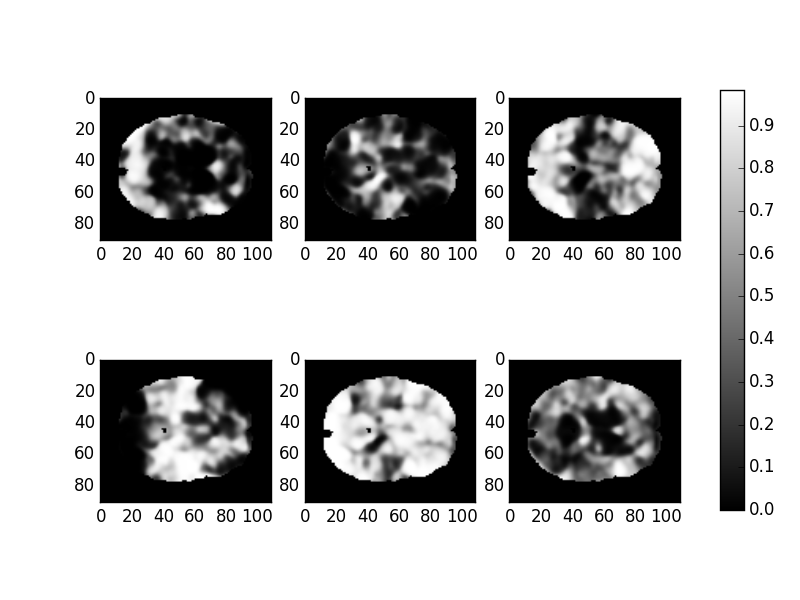
\includegraphics[scale=0.35]{dct_p_map}
  \caption{p Map}
\end{subfigure}%
\begin{subfigure}{.5\textwidth}
  \centering
  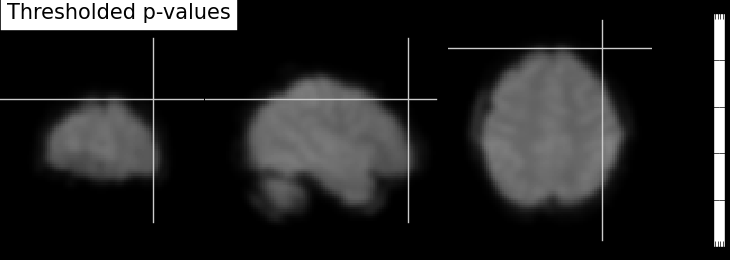
\includegraphics[scale=0.35]{dct_sig_p_map}
  \caption{Significant p Map} 
\end{subfigure}
\caption{DCT Model Parametric Maps\label{fig:dctMF}}
\end{figure}

